\documentclass[xcolor={table}, aspectratio=169]{beamer}
%
% Choose how your presentation looks.
%
% For more themes, color themes and font themes, see:
% http://deic.uab.es/~iblanes/beamer_gallery/index_by_theme.html
%
\defbeamertemplate{footline}{my frame number}
{
    \hfill
    \usebeamercolor[fg]{page number in head/foot}
    \usebeamerfont{page number in head/foot}
    \raisebox{0.25cm}[0pt][0pt]{
        \insertframenumber\kern1em}
}
\mode<presentation>
{
    \usetheme{default}
    \usecolortheme{seagull}
    \usepackage{csquotes}
    % \usefonttheme{default}
\usefonttheme[onlymath]{serif}
    \setbeamertemplate{caption}[numbered]
    \setbeamertemplate{footline}[my frame number]
    \setbeamertemplate{navigation symbols}{}
    \addtobeamertemplate{frametitle}{\vskip+0.5ex}{}
}
% \AtBeginSection[] {
%     \begin{frame}<beamer>
%     \frametitle{Outline}
%     \tableofcontents[currentsection]
%     \end{frame}
% }
% \AtBeginSubsection[] {
%     \begin{frame}<beamer>
%     \frametitle{Outline}
%     \tableofcontents[currentsection, currentsubsection]
%     \end{frame}
% }

\usepackage[english]{babel}
\usepackage[export]{adjustbox}
\usepackage[permil]{overpic}
\usepackage{threeparttable}
\usepackage{graphicx}
\usepackage{subcaption}
\usepackage{setspace}
\usepackage{ulem}
\usepackage{amssymb}
\usepackage{subcaption}
\usepackage{psfrag}
%\usepackage{natbib}
\usepackage[autocite=superscript,backend=bibtex, style=authoryear]{biblatex}
\addbibresource{refs.bib}

\usepackage{multirow}
\usepackage{hyperref}
\usepackage{graphicx}
\usepackage{color}
% \usepackage{cleveref}
\usepackage[font=scriptsize]{caption}
\usepackage{booktabs}
\usepackage{amsmath}
\usepackage{tikz}
\usepackage{siunitx}
\usepackage{tikz}
\usetikzlibrary{arrows.meta, calc}

\definecolor{slidebg}{HTML}{171717}
\definecolor{sdfgreen}{HTML}{16803D}
\definecolor{advred}{HTML}{DC2626}
\definecolor{lossgray}{HTML}{64748B}

\sisetup{output-exponent-marker=\ensuremath{\mathrm{e}}}



%\usepackage{fontspec}

\graphicspath{{stevens/}{figures/}}

\makeatletter
\def\beamer@framenotesbegin{% at beginning of slide
     \usebeamercolor[fg]{normal text}
      \gdef\beamer@noteitems{}%
      \gdef\beamer@notes{}%
}
\makeatother

\usebackgroundtemplate
{
    \begin{tabular}{@{}c@{}}
        
\includegraphics[width=\paperwidth]{presentation_top.png} \\
        \rule{0pt}{0.74\paperheight} \\
        
\includegraphics[width=\paperwidth]{presentation_bottom.png}
    \end{tabular}
}

\vspace{1cm}

\title[Lit Review]
      {Deep Learning in Asset Pricing}

\author[Author] % (optional, use only with lots of authors)
{Luyang Chen, Markus, Pleger, Jason Zhu}
% - Use the \inst{?} command only if the authors have different
%   affiliation.

\institute[Stevens Institute] % (optional, but mostly needed)
{
	Presented by: Andre Sealy\\
  Finance 705\\
  Stevens Institute of Technology\\
%System description details at \cite{w2020shift}}
}
\date{\\
{\footnotesize \today}}

\subject{Talk at Venue}


%\author[Ionut Florescu]{\texorpdfstring{\footnotesize Ionu\c{t} Florescu \\
%       \vspace*{0.5\baselineskip}
%     {\footnotesize Committee: \\
%      Dr. George Calhoun, Dr. Dragoș Bozdog, \\
%      Dr. Emmanuel Hatzakis, Dr. Rupak Chatterjee}}{Ionu\c{t} Florescu}}
% \institute{\footnotesize Financial Engineering}
% \date{{\footnotesize September 12, 2020}}

\begin{document}

{
\setbeamertemplate{footline}{}
\usebackgroundtemplate
{
	\begin{tabular}{@{}c@{}}
		\begin{overpic}[width=\paperwidth]{title_top.png}
			\put(25,-35){
\includegraphics[height=0.15\paperheight]{title_logo.png}}
		\end{overpic} \\
		\rule{0pt}{0.74\paperheight}                     \\
		
\includegraphics[width=\paperwidth]{title_bottom.png}
	\end{tabular}
}

\begin{frame}

	\titlepage

\end{frame}
}

\begin{frame}{Background}

Traditional asset pricing models, such as the Capital Asset Pricing Model (CAPM) and Fama–French factor models, seek to explain differences in expected stock returns through exposure to systematic risk. However, these models typically impose restrictive functional forms and rely on a predetermined set of risk factors.

\end{frame}

\begin{frame}{Research Questions}

  This paper attempts to answer the following: Can deep learning improve the estimation of the stochastic discount factor and explain differences in expected stock returns?

\end{frame}

\begin{frame}{Model Innovations}

  The model formalizes a deep neural network that estimates an asset pricing model for individual stock returns. This estimation rests on three innovations:

  \vspace{0.3cm}
  \begin{itemize}
    \item The fundamental no-arbitrage condition
    \vspace{0.3cm}
    \item An adversial approach for testing assets
    \vspace{0.3cm}
    \item Economics states extracted from macroeconomic time series.
    
  \end{itemize}

\end{frame}

\begin{frame}
	\centering
	\vfill
	{\Large \textbf{No-Arbitrage Asset Pricing}}
	\vfill
\end{frame}

\begin{frame}{No-Arbitrage Asset Pricing}

  Let $R_{t+1}$ denote return of asset $i$ at time $t+1$. The no-arbitrage assumption is the stochastic discount factor (SFD) $M_{t+1}>0$, for any excess returns $R_{t+1,i}^e=R_{t+1,i}-R_{t+1}^f$, we have

  \[\mathbb{E}_t\left[M_{t+1}R_{t+1,i}^e\right]=0\iff \mathbb{E}\left[R_{t+1,i}^e\right]=\underbrace{\left(-\frac{\text{Cov}_t\left(R_{t+1,i}^e,M_{t+1}\right)}{\text{Var}_t(M_{t+1})}\right)}_{\beta_{t,i}}\cdot\underbrace{\frac{\text{Var}_t(M_{t+1})}{\mathbb{E}_t\left[M_{t+1}\right]}}_{\lambda_t}\]

  where $\beta_{t,i}$ is the exposure to systematic risk and $\lambda_t$ is the price of risk. 

\end{frame}

\begin{frame}{No-Arbitrage Asset Pricing}

  We define the SDF as the following

  \[
  M_{t+1}=1\sum_{i=1}^N\omega_{t,i}R_{t+1,i}^e=1-\omega_t^\top R_{t+1}^e.
  \]

  Since $\mathbb{E}\left[R_{t+1}^eM_{t+1}\right]=0$ implies the SDF weights 

  \[\omega_t=\mathbb{E}_t\left[R_{t+1}^e(R^e_{t+1})^\top\right]^{-1}\mathbb{E}\left[R_{t+1}^e\right]\].

  These are the portfolio weights of the coniditional mean-variance on the efficient portfolio.

\end{frame}

\begin{frame}{No-Arbitrage Asset Pricing}

  Let $F_{t+1}=\omega_t^\top R_{t+1}^e$  be the portfolio tangent to the efficiency frontier. Then we can rewrite the equation as the following

  \[
  \mathbb{E}\left[R_{t+1,i}^e\right]=\frac{\text{Cov}_t\left(R_{t+1,i}^e,F_{t+1}\right)}{\text{Var}_t(F_{T+1})}\cdot\mathbb{E}_t\left[F_{t+1}\right]=\beta_{t,i}\mathbb{E}_t\left[F_{t+1}\right]
  \]

  So the no-arbitrage implies a one-factor model

  \[R_{t+1,i}^e=\beta_{t,i}F_{t+1}+\epsilon_{t+1,i}\]

  where $\mathbb{E}\left[\epsilon_{t+1,i}\right],\text{Cov}_t\left(F_{t+1},\epsilon_{t+1,i}\right)=0$.


\end{frame}

\begin{frame}
	\centering
	\vfill
	{\Large \textbf{Generative Adversarial Methods}}
	\vfill
\end{frame}

\begin{frame}{Generative Adversarial Methods}

  Let $g(\cdot):\mathbb{R}^p\times\mathbb{R}^D$, where $I_t\times I_{t,i}\in\mathbb{R}^p\times\mathbb{R}^q$ denotes all the variables in the information set at time $t$ and $D$ is the number of moment conditions. Then the conditional no-arbitrage moment condition can be defined as the following:

  \[
  \mathbb{E}\left[M_{t+1}R_{t+1,i}^eg(I_t,I_{t,i})\right]=0,
  \]
  where $I_t$ denotes $p$ macroeconomic conditioning variables that are not asset specific, and $I_{t,i}$ are $q$ firm-specific characteristics. 

\end{frame}

\begin{frame}{Generative Adversarial Methods}

  The paper uses a theoritical adversarial approach to select the moment conditions that lead to the largest mispricings:

  \[
  \underset{\omega}{\min}\;\underset{g}{\max}\frac{1}{N}\sum_{j=1}^{N}\left\| \mathbb{E}\left[\left( 1-\sum_{i=1}^N\omega(I_t,I_{t,i})R_{t+1,i}^e \right)R_{t+1,j}^eg(I_t,I_{t,j}) \right] \right\|^2
  \]
  where the function $\omega$ and $g$ are trained in a neural network. 

\end{frame}

\begin{frame}{Generative Adversarial Method}

  \begin{figure}
     \centering
    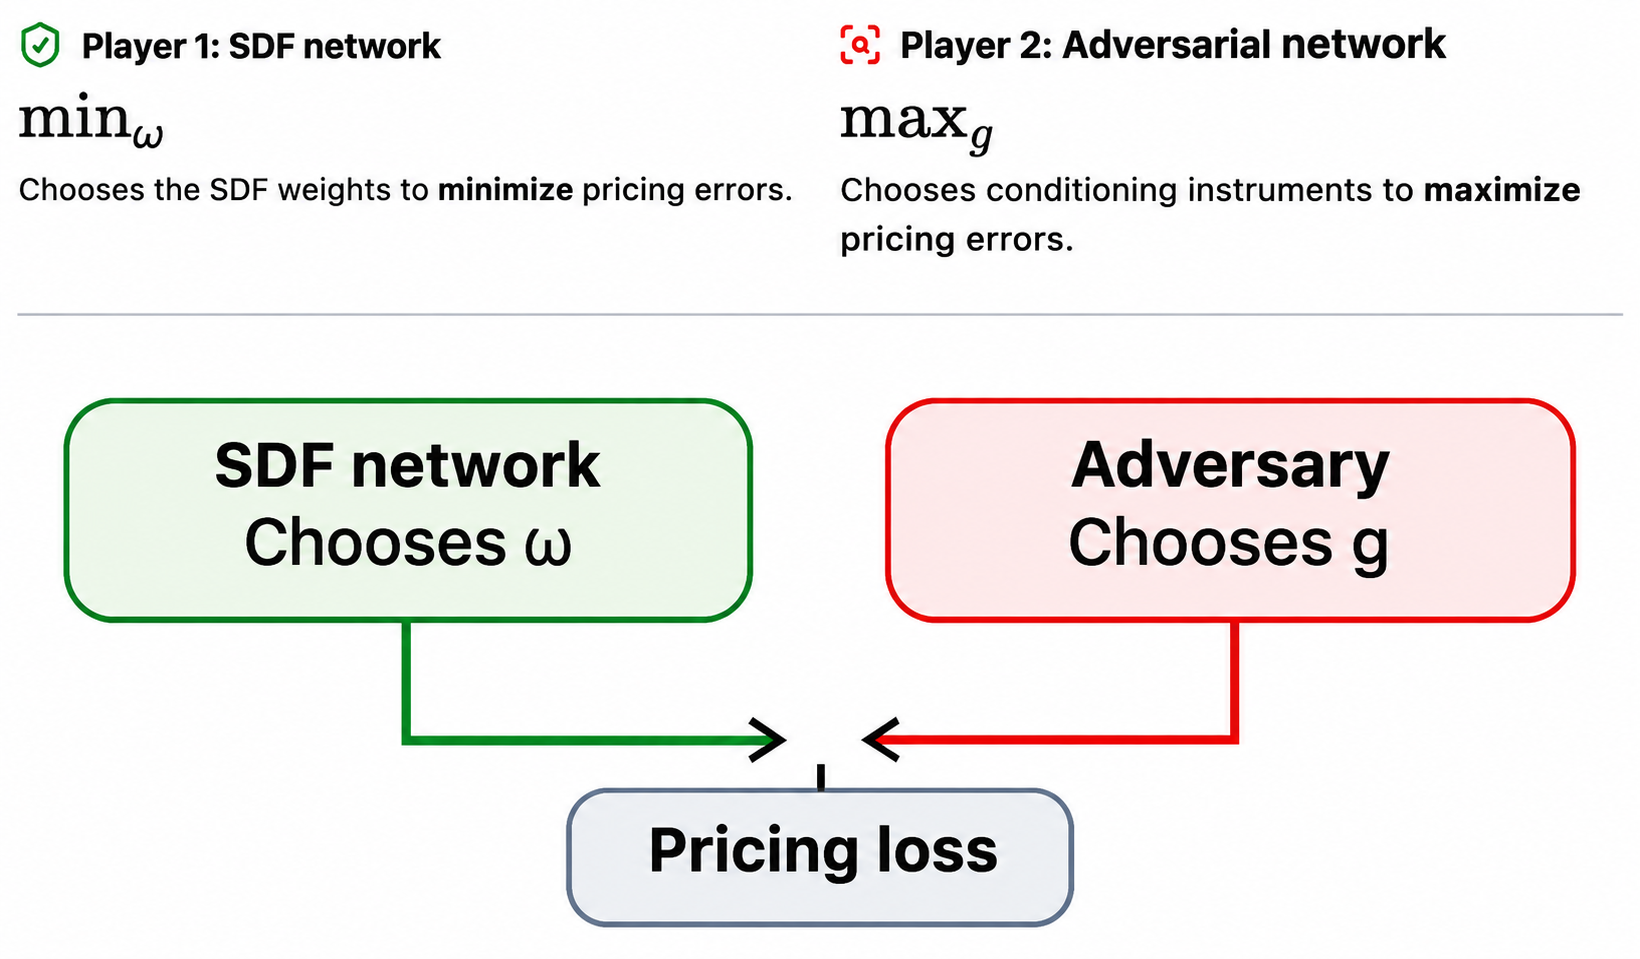
\includegraphics[width=0.7\linewidth]{pics/loss_diagram.png}
  \caption{Adversarial Pricing Loss Diagram}
  \label{fig:}
  \end{figure}

\end{frame}

%%% -------------------------------------------------------

\begin{frame}{Generative Adversarial Method}

  The empirical loss function minimizes the weighted sample moments and specifics how the SDF network measures pricing errors.

  \[L\left(\omega\mid\hat{g},I_t,I_{t,i}\right)=\frac{1}{N}\sum_{i=1}^N\frac{T_i}{T}\left\|\frac{1}{T_i}\sum_{t\in T_i}M_{t+1}R_{t+1,i}^e\hat{g}(I_t,I_{t,i})\right\|^2\]


\end{frame}

\begin{frame}
	\centering
	\vfill
	{\Large \textbf{Model Architecture}}
	\vfill
\end{frame}


\begin{frame}{GAN Model Architecture}
  \centering
  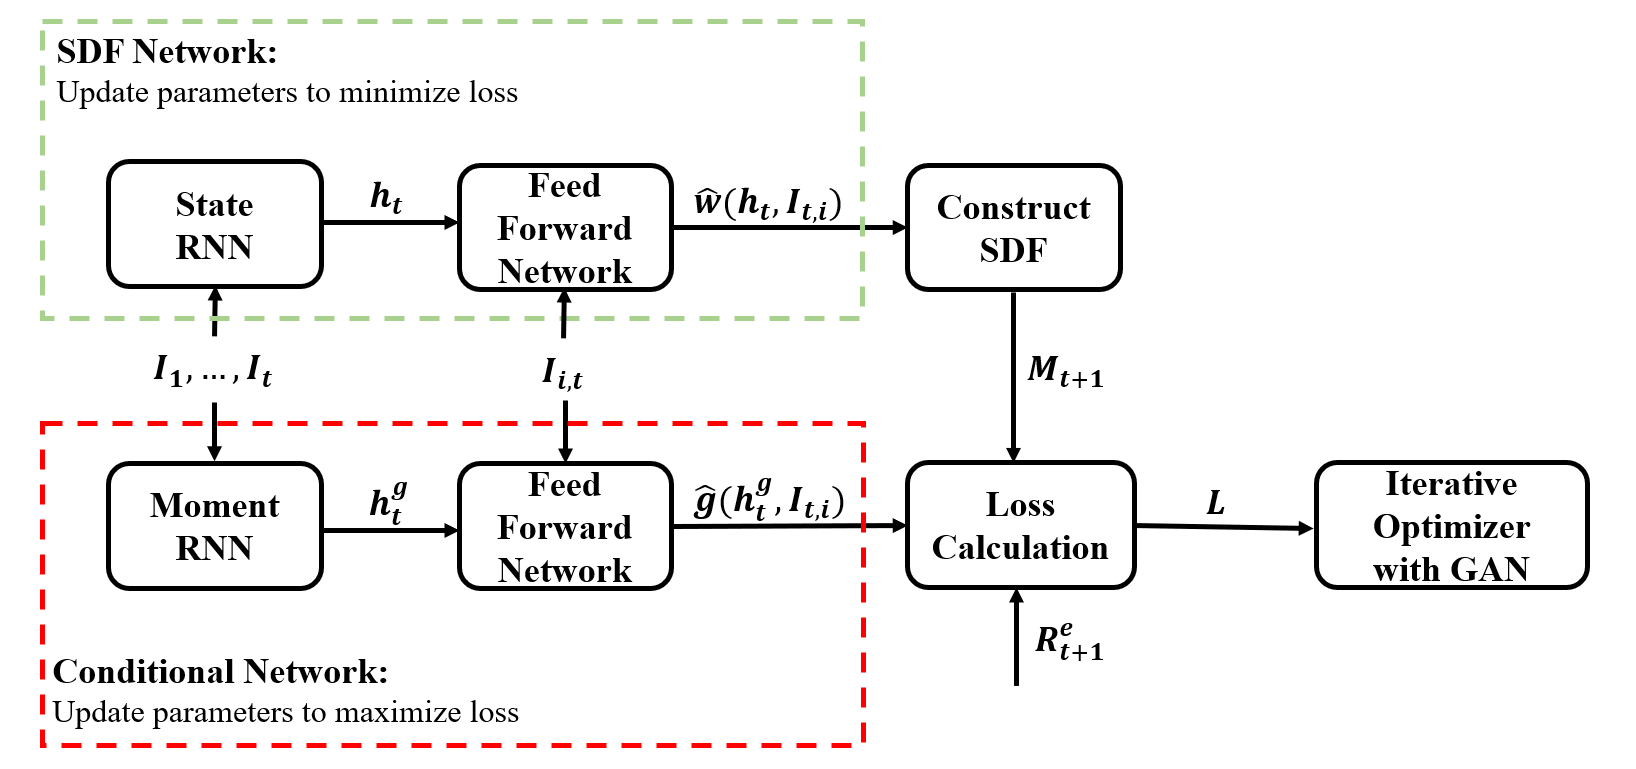
\includegraphics[width=\linewidth,height=.62\textheight,keepaspectratio] {pics/gan-model-architecture.png}\par
  \smallskip
  {\scriptsize Figure 1 from Chen, Pelger, and Zhu,
  \emph{Deep Learning in Asset Pricing}
  (\href{https://ssrn.com/abstract=3350138}{SSRN 3350138}).\par}
\end{frame}


\begin{frame}{RNN with LSTM}
  \begin{figure}
     \centering
    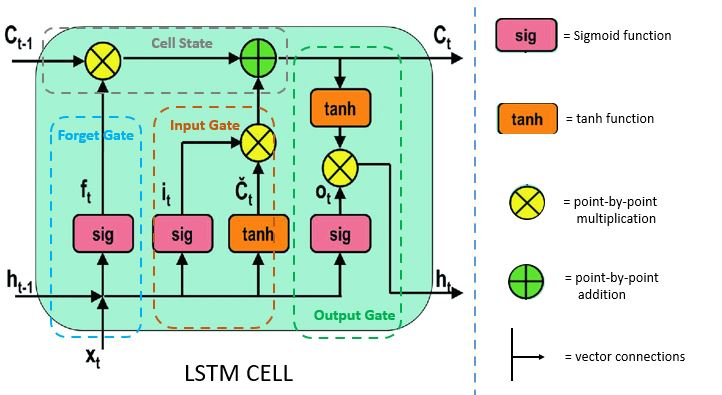
\includegraphics[width=0.7\linewidth]{pics/lstm.JPG}
  \caption{Long short-term memory}
  \end{figure}

\end{frame}


\begin{frame}{LSTM: General Mathematical Framework}

\footnotesize
\setlength{\abovedisplayskip}{4pt}
\setlength{\belowdisplayskip}{4pt}

\begin{columns}[T,onlytextwidth]

% ==========================================
% LEFT COLUMN: MATHEMATICAL FRAMEWORK
% ==========================================
\begin{column}{0.68\textwidth}

\textbf{1. Input Layer}
\[
x_t\in\mathbb{R}^{p},\quad
h_{t-1},c_{t-1}\in\mathbb{R}^{d}
\]
\[
u_t=[h_{t-1};x_t]
\]

\vspace{0.1cm}

\textbf{2. LSTM Gates}
\[
\begin{aligned}
f_t &= \sigma(W_f u_t+b_f),\\
i_t &= \sigma(W_i u_t+b_i),\\
o_t &= \sigma(W_o u_t+b_o)
\end{aligned}
\]

\vspace{0.1cm}

\textbf{3. Memory Update}
\[
\begin{aligned}
\tilde{c}_t
&=\tanh(W_c u_t+b_c),\\
c_t
&=f_t\odot c_{t-1}
+i_t\odot\tilde{c}_t
\end{aligned}
\]

\vspace{0.1cm}

\textbf{4. Hidden State Output}
\[
\boxed{
h_t=o_t\odot\tanh(c_t)
}
\]

\end{column}

% ==========================================
% RIGHT COLUMN: NOTATION
% ==========================================
\begin{column}{0.29\textwidth}

\textbf{Notation}

\vspace{0.15cm}

\begin{itemize}
    \setlength{\itemsep}{0.18cm}

    \item $x_t$:
    Input vector

    \item $h_t$:
    Hidden state

    \item $c_t$:
    Memory cell

    \item $f_t$:
    Forget gate

    \item $i_t$:
    Input gate

    \item $o_t$:
    Output gate

    \item $W,b$:
    Weights and biases

    \item $\sigma$:
    Sigmoid function

    \item $\odot$:
    Element-wise product

\end{itemize}

\end{column}

\end{columns}

\end{frame}

\begin{frame}{LSTM - Examples of Macroeconomic Indicators}

  \begin{figure}
     \centering
    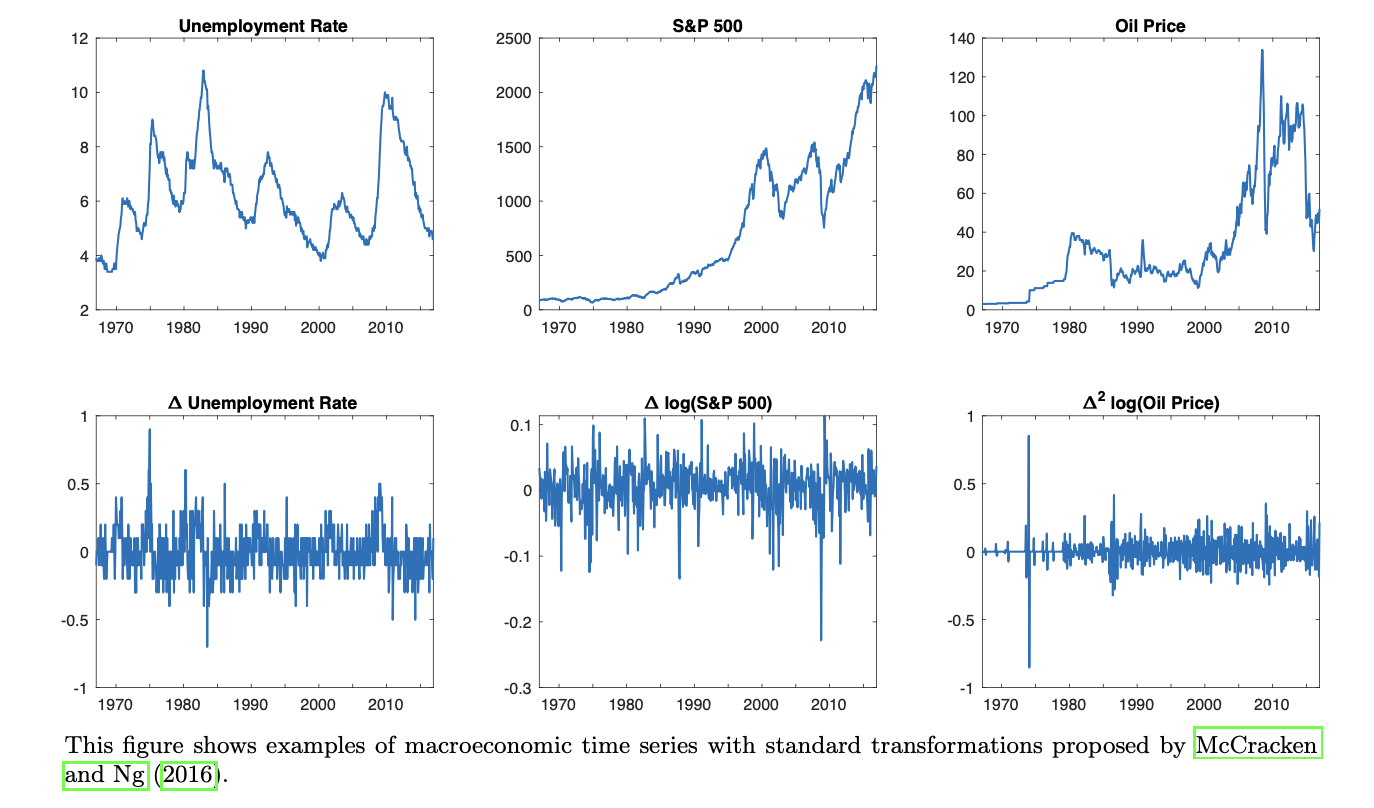
\includegraphics[width=0.8\linewidth]{pics/macro.png}
  \caption{Examples of Macroeconomic Variables}
  \end{figure}

\end{frame}


\begin{frame}{LSTM Architecture Comparison}

\small
\setlength{\tabcolsep}{6pt}
\renewcommand{\arraystretch}{1.3}

\begin{table}[htbp]
\centering

\begin{tabular}{lcc}
\hline
\textbf{Component} &
\textbf{SDF Network} &
\textbf{Conditional Network} \\
\hline

Input dimension $p$ & 178 & 178 \\

Hidden-state dimension $d$ & 4 & 32 \\

LSTM output &
$h_t \in \mathbb{R}^{4}$ &
$h_t^g \in \mathbb{R}^{32}$ \\

Next component &
SDF FFN &
Conditional FFN \\

Training objective &
Minimize loss &
Maximize loss \\

\hline
\end{tabular}

\vspace{0.2cm}

\caption{Comparison of the LSTM architectures used
in the SDF and conditional networks of Chen,
Pelger, and Zhu (2021).}

\label{tab:lstm_comparison}

\end{table}

\end{frame}


\begin{frame}{Feed Forward Network}

  \begin{figure}
     \centering
    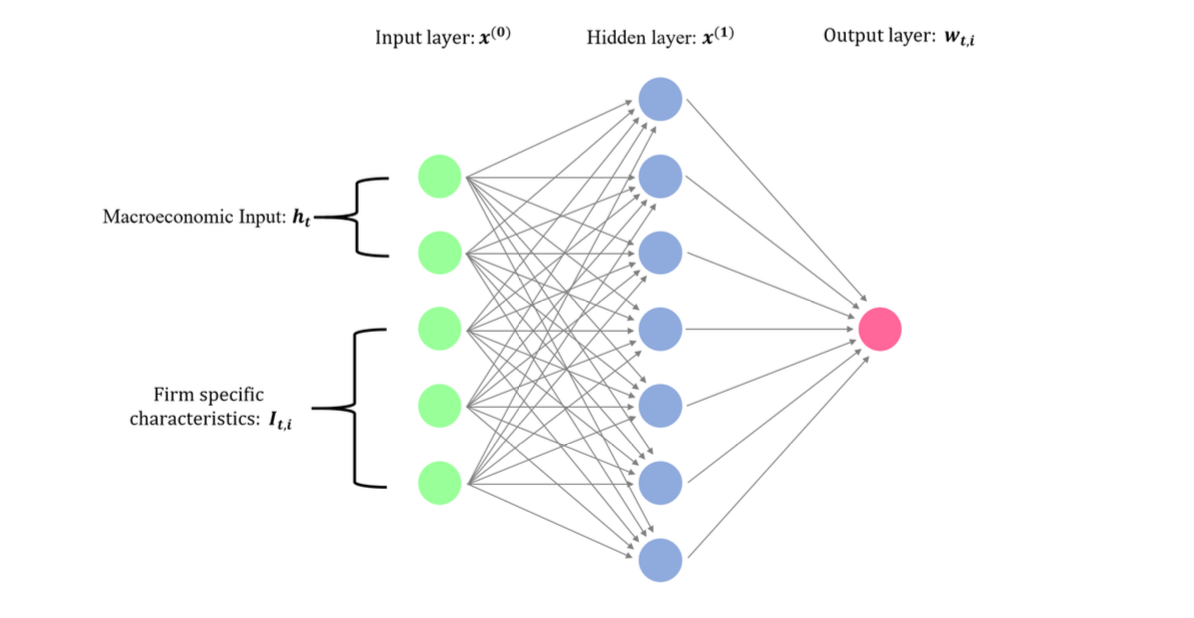
\includegraphics[width=0.8\linewidth]{pics/FFN.png}
  \caption{Feedfoward Network with Single Hidden Layer}
  \end{figure}

\end{frame}

%%% -------------------------------------------------------

\begin{frame}{Feedforward Neural Network: General Framework}

\small
\setlength{\abovedisplayskip}{5pt}
\setlength{\belowdisplayskip}{5pt}

\begin{columns}[T,onlytextwidth]

% ==========================================
% LEFT COLUMN: MATHEMATICAL FRAMEWORK
% ==========================================
\begin{column}{0.68\textwidth}

\textbf{1. Input Layer}
\[
x^{(0)}=x\in\mathbb{R}^{d_0}
\]

\vspace{0.15cm}

\textbf{2. Hidden Layers} ($\ell=1,\ldots,L$)
\[
\boxed{
x^{(\ell)}
=
\sigma\left(
W^{(\ell)}x^{(\ell-1)}+b^{(\ell)}
\right)
}
\]

\vspace{0.15cm}

\textbf{3. Output Layer}
\[
\boxed{
\hat{y}
=
\phi\left(
W^{(L+1)}x^{(L)}+b^{(L+1)}
\right)
}
\]

\vspace{0.15cm}

\textbf{4. Parameter Estimation}
\[
\hat{\theta}
=
\arg\min_{\theta}\mathcal{L}(\theta)
\]

\end{column}

% ==========================================
% RIGHT COLUMN: NOTATION
% ==========================================
\begin{column}{0.29\textwidth}

\textbf{Notation}

\vspace{0.2cm}

\begin{itemize}
    \setlength{\itemsep}{0.35cm}

    \item $W^{(\ell)}$:
    Weight matrix

    \item $b^{(\ell)}$:
    Bias vector

    \item $\sigma$:
    Hidden activation (ReLU)

    \item $\phi$:
    Output activation

    \item $L$:
    Number of hidden layers

\end{itemize}

\end{column}

\end{columns}

\end{frame}



\begin{frame}{Feedforward Neural Network Comparison}

\small
\setlength{\tabcolsep}{6pt}
\renewcommand{\arraystretch}{1.20}

\begin{table}[htbp]
\centering

\begin{tabular}{lcc}
\hline
\textbf{Component} &
\textbf{SDF Network} &
\textbf{Conditional Network} \\
\hline

Input dimension $d_0$ & 50 & 78 \\

Macroeconomic states & 4 & 32 \\

Firm characteristics & 46 & 46 \\

Hidden layers $L$ & 2 & 0 \\

Neurons per hidden layer & 64 & N/A \\

Output dimension & 1 & 8 \\

Network output &
$\omega_{t,i}$ & $g_{t,i}$ \\

Optimization &
Minimize loss & Maximize loss \\

\hline
\end{tabular}

\vspace{0.2cm}

\caption{Comparison of the feedforward neural network
architectures used in the SDF and conditional networks
of Chen, Pelger, and Zhu (2021).}

\label{tab:ffn_comparison}

\end{table}

\end{frame}

\begin{frame}
	\centering
	\vfill
	{\Large \textbf{Data}}
	\vfill
\end{frame}

\begin{frame}{Data Overview}

\small
\centering
\setlength{\tabcolsep}{4pt}
\renewcommand{\arraystretch}{1.6}

\begin{table}[htbp]
\centering

\begin{tabular}{
    p{0.25\textwidth}
    p{0.31\textwidth}
    p{0.35\textwidth}
}
\hline
\textbf{Data} &
\textbf{Source} &
\textbf{Description} \\
\hline

Stock returns &
CRSP &
Monthly U.S. equity returns \\

Firm characteristics &
CRSP/Compustat &
46 stock-specific characteristics \\

Marco variables &
FRED-MD and other sources &
178 monthly time series \\

Risk-free rate &
Kenneth French Data Library &
One-month Treasury bill rate \\

\hline
\end{tabular}

\vspace{0.25cm}

\caption{Overview of the datasets used in Chen, Pelger,
and Zhu (2021). The sample covers U.S. equities from
January 1967 to December 2016.}

\label{tab:data_overview}

\end{table}

\end{frame}


\begin{frame}{Time Split Training}
  
  \begin{figure}
     \centering
    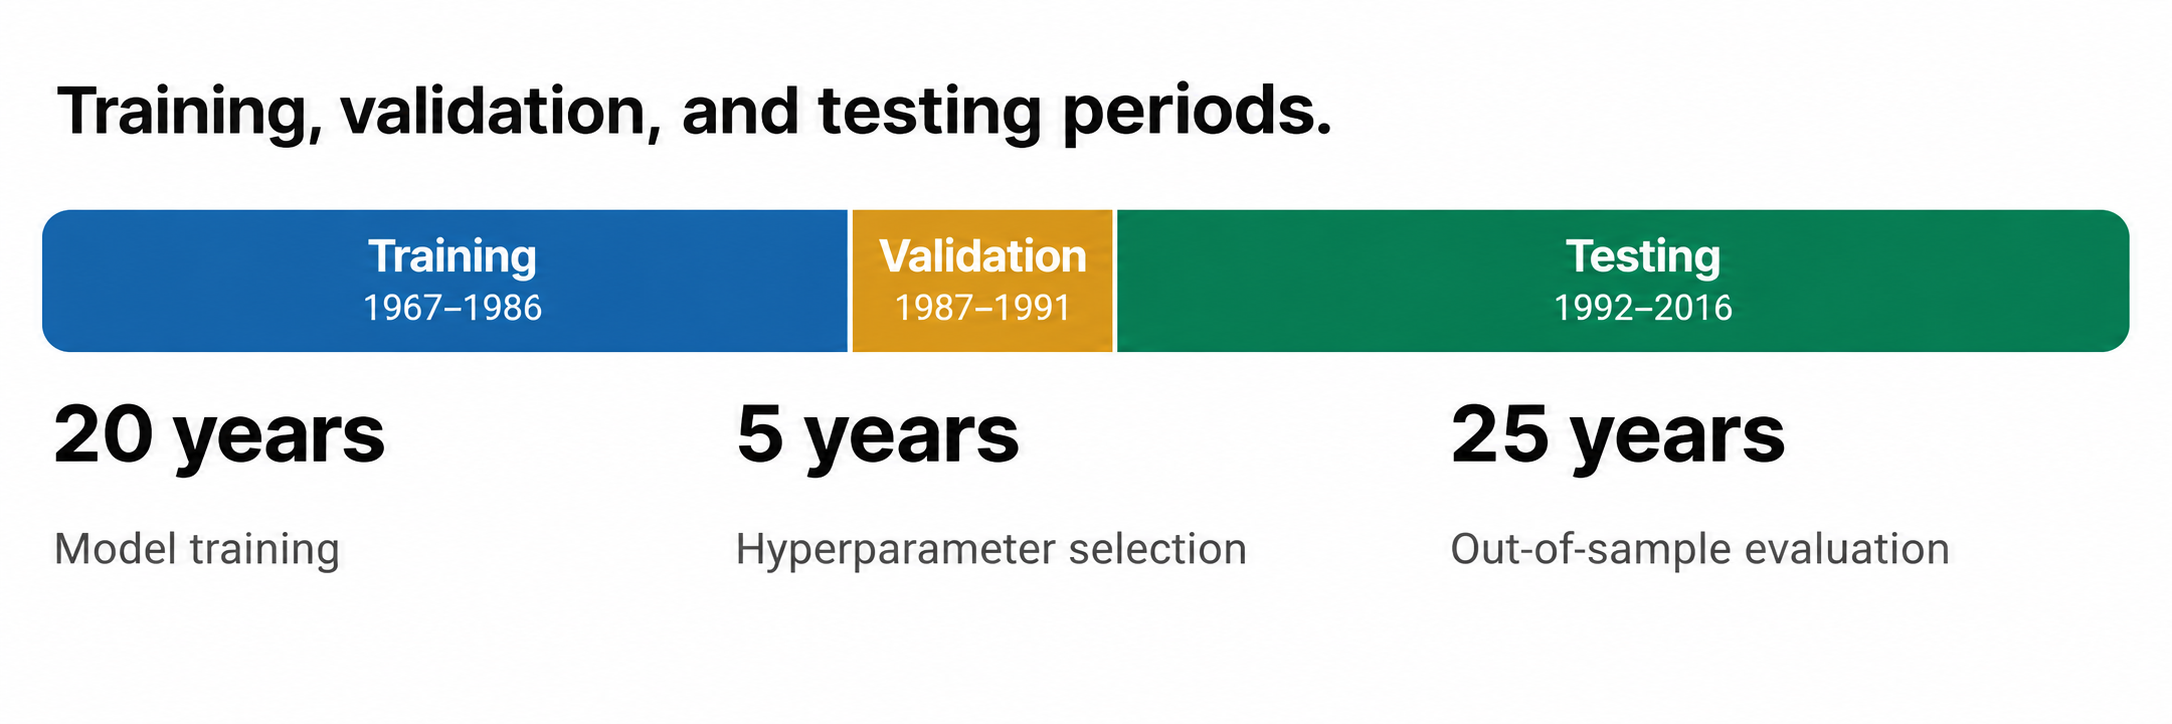
\includegraphics[width=\linewidth]{pics/model_training.png}
  \end{figure}

\end{frame}

%%% -------------------------------------------------------


\begin{frame}
	\centering
	\vfill
	{\Large \textbf{Performance}}
	\vfill
\end{frame}


\begin{frame}{GAN Illustration}

  \begin{figure}
     \centering
    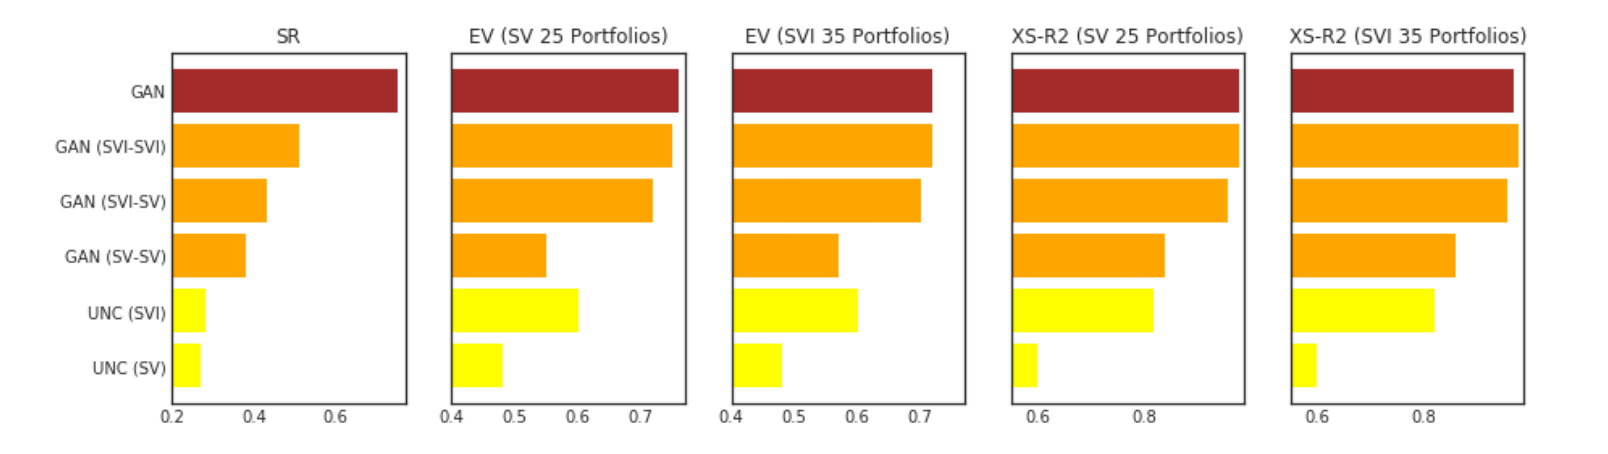
\includegraphics[width=\linewidth]{pics/gan.png}
  \caption{GAN Illustration, from Chen, Pelger, and Zhu (2021), demonstrates how adversarially selecting test assets improves the performance of a stochastic discount factor (SDF) compared with estimating an SDF using unconditional pricing restrictions.}
  \end{figure}
  


\end{frame}

%%% -------------------------------------------------------

\begin{frame}{GAN Performance}

  \begin{figure}{}
     \centering
    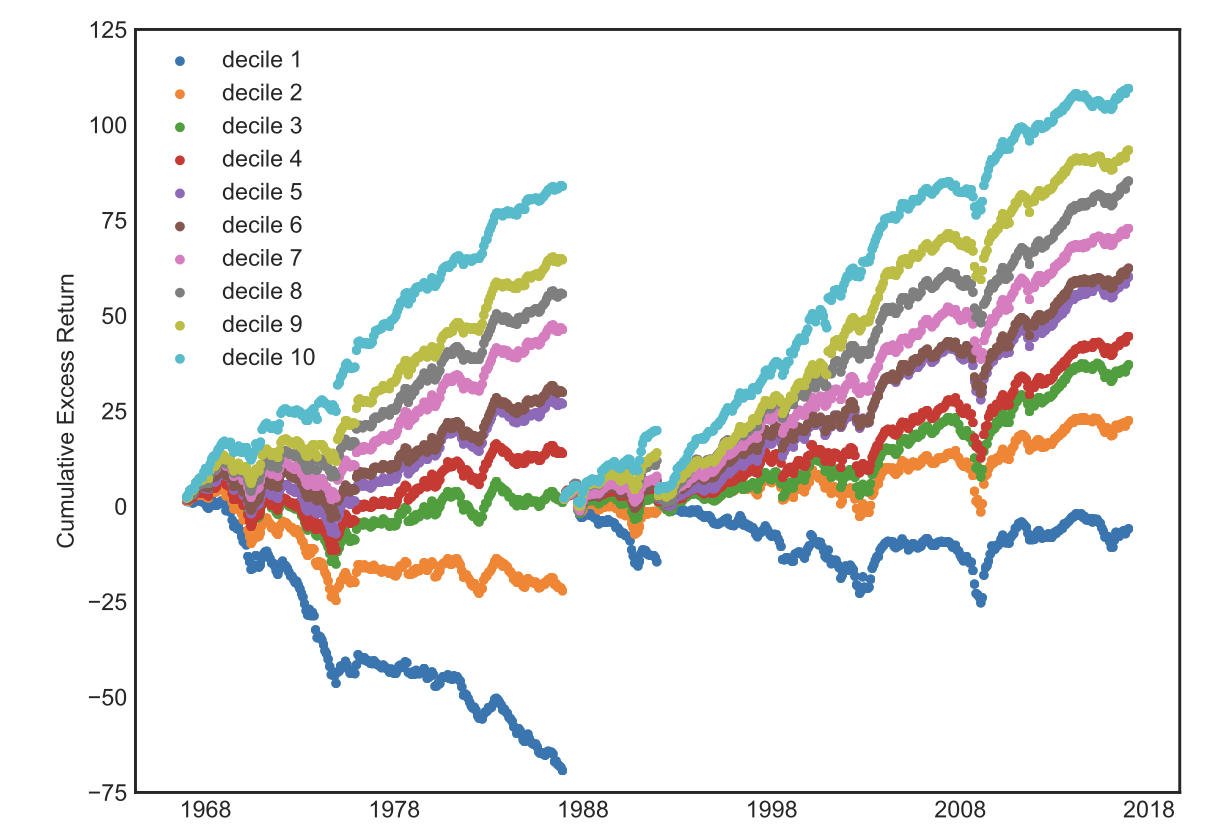
\includegraphics[width=0.6\linewidth]{pics/cum_returns.png}
  \caption{Cumulative Excess Returns of Decile Sorted Portfolios with GAN}
  \end{figure}

\end{frame}

%%% -------------------------------------------------------

\begin{frame}{Pricing Errors}

  \begin{figure}
     \centering
    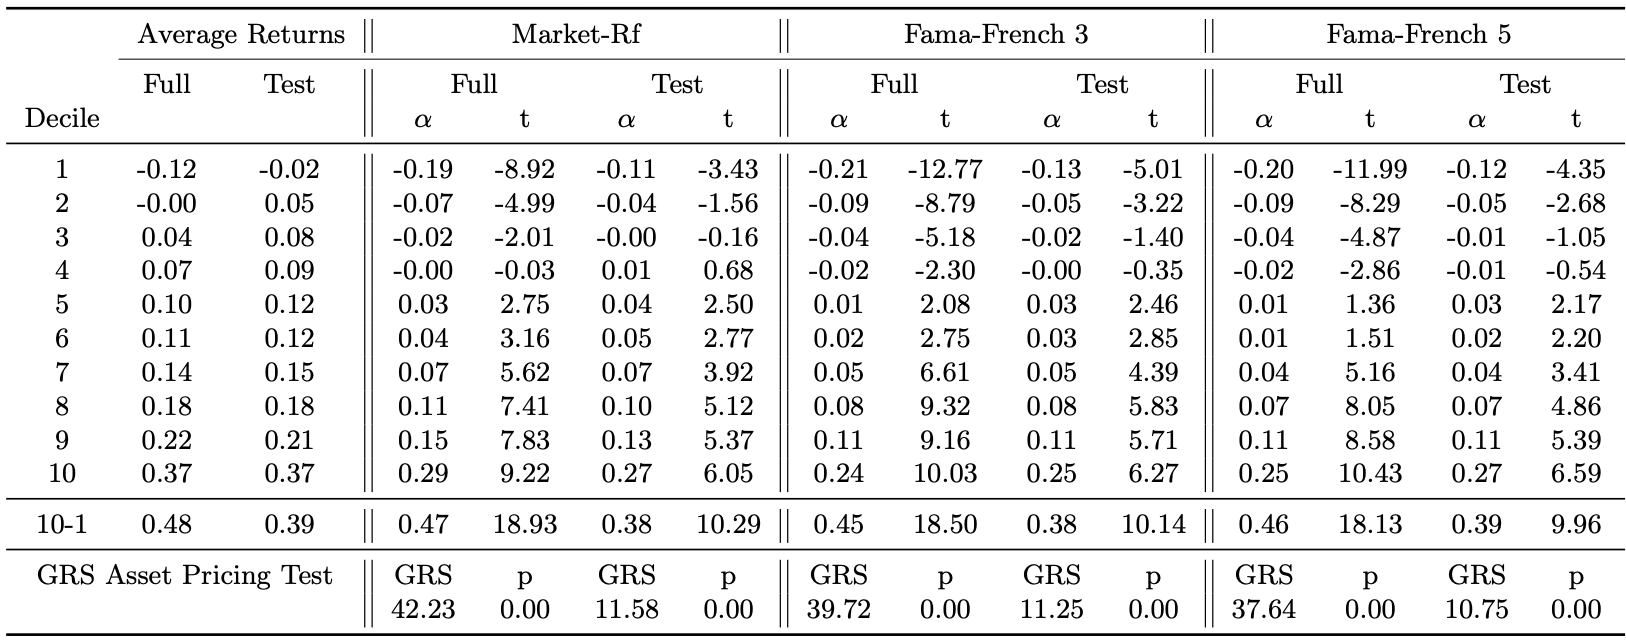
\includegraphics[width=0.9\linewidth]{pics/Pricing Errors.png}
  \caption{Time Series Pricing Errors for $\beta$-Sorted Portfolios}
  \end{figure}

\end{frame}

%%% -------------------------------------------------------

\begin{frame}{Explained Variation}

  \begin{figure}{}
     \centering
    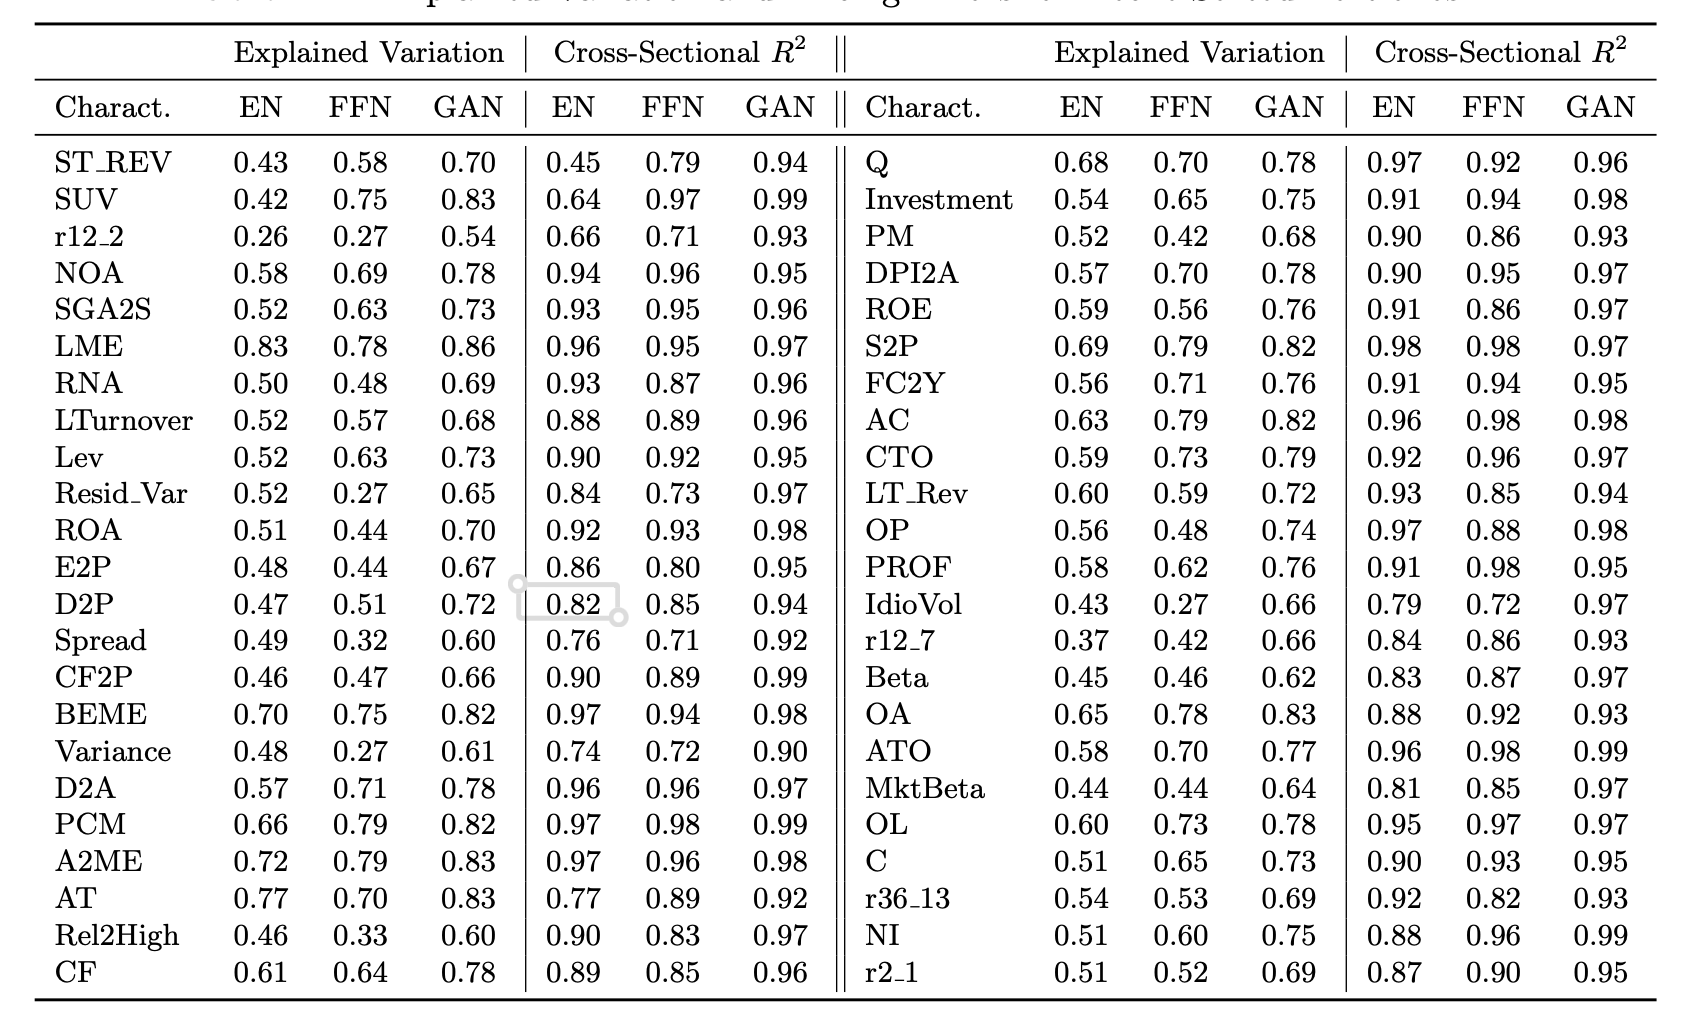
\includegraphics[width=0.8\linewidth]{pics/ev.png}
  \caption{Explained Variation and Pricing Errors for Decile Sorted Portfolios}
  \end{figure}

\end{frame}

%%% -------------------------------------------------------

\end{document}
